\documentclass{beamer}
\usetheme{default}
\usepackage{microtype}
\usepackage{graphicx}
\title{The Role of Bartle’s Gamer Types in Gamified Higher Education}
\author{William Seymour}
\institute{University of Warwick}
\date{March 12th, 2015}
\beamertemplatenavigationsymbolsempty

\begin{document}
	\begin{frame}
		\titlepage
	\end{frame}
	\frame{
		\frametitle{Presentation Overview}
		\begin{enumerate}
			\item What is gamification?
			\item What are Bartle's gamer types?
			\item Research undertaken
			\item Conclusion and further work
			\item Project evaluation
		\end{enumerate}
	}
	
	\frame{
		\frametitle{Gamification}
		\begin{quotation}
			``The use of game design elements \\ in non-game contexts''\footnote{Definition from “From game design elements to gamefulness by Detarding et al. (2011)}
		\end{quotation}
		
		Or, put another way, transplanting the game mechanics that make games engaging into other media with the aim of driving engagement.
		\newline
		
		It is important here to make the distinction between \textit{games} and \textit{gamified activities}. Not interested in things like controller support or fancy 3D graphics that typify game experiences.
	}
	
	\frame{
		\frametitle{Gamification}
		Though it existed since 2002, the term really spiked in usage from \textasciitilde2010\footnote{Google Trends image: proportion of gamification searches relative to the peak}. Gamification has psychological roots in operant conditioning (cf. B. F. Skinner) and Self Determination Theory.
		
			\begin{figure}
				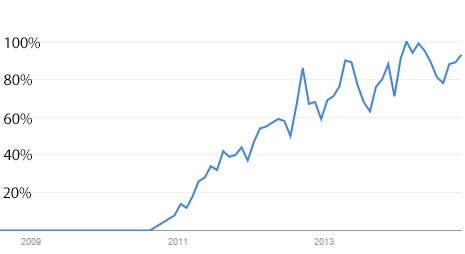
\includegraphics[width=0.5\linewidth]{../img/usage-graph.png}
			\end{figure}
			
			Usage of time over skill as a method of determining worth makes all players feel involved instead of just the top few.
	}
	
	\frame{
		\frametitle{Learning Analytics}
		The concept of using data analysis to inform the education process, giving a more personalised experience for students. Makes it possible to match students together by ability or learning style.
		\newline
		
		More popular than gamfication in HE, possibly due to the rise of big data.
		
		\begin{figure}
			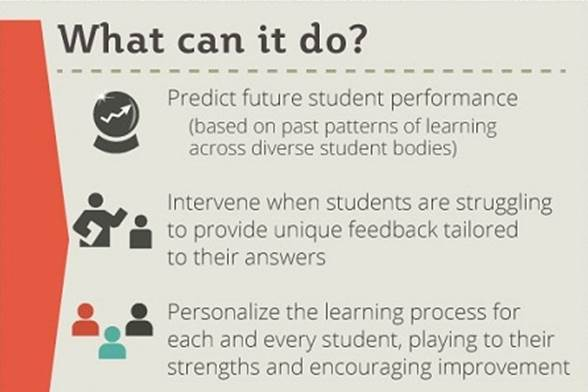
\includegraphics[width=0.6\linewidth]{../img/infographic.jpg}
			\footnote{Image part of an infographic by www.opencolleges.edu.au}
		\end{figure}
	}
	
	\frame{
		\frametitle{What does gamified higher education look like?}

		Uses a combination of gamification and learning analytics to enrich all aspects of campus life - from learning to sport and healthy eating.
		\newline
		
		We already have mechanisms for tracking visits to food outlets, so why not extend that and reward students for eating healthily? What data can we get from student cards and SSO?
		
		\begin{figure}
			
\includegraphics[width=0.5\linewidth]{../img/horizon.png}
		\end{figure}
		
		Would students be more inclined to study if they knew everyone else was putting in more effort?		
	}
	
	\frame{
	\frametitle{Bartle's Gamer Types}
	
	Proposed by Richard Bartle in his 1996 paper, the model categorises players into Socialisers, Killers, Achievers and Explorers. It acts as a way of psychologically profiling gamers based on their thoughts and actions in-game.
	
	\begin{center}
	\begin{tabular}{|c|c|c|}
		\hline - & Acting & Interacting \\ 
		\hline Players & Killers & Socialisers \\ 
		\hline World & Achievers & Explorers \\ 
		\hline 
	\end{tabular} 
	\end{center}
	
	Bartle refined this model in a later paper, but as only explicit and implicit variants of the above roles were added, along with adjustments for players changing over time, the project focuses on the simpler version.
	
	}
	
	\frame{
	\frametitle{Bartel's Gamer Types}	
		Bartle types can be used to reason about ecosystems of players in online multiplayer games. For example, the effect on the player base of increasing one type of user can be seen below.\footnote{Image from ``Hearts, clubs, diamonds, spades'' by Richard Bartle (1996).}
		\newline
		
		Despite being designed for MUDs (and by extension, MMOs), the Bartle types have found their way into a large amount of books and papers on gamification.
		
		\begin{figure}
			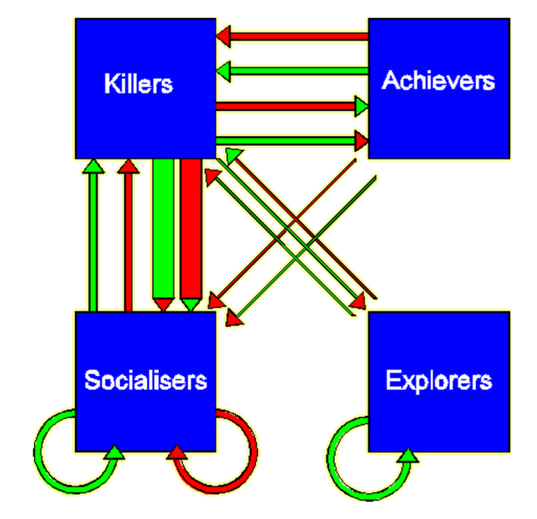
\includegraphics[width=0.5\linewidth]{../img/bartle.png}
		\end{figure}
	}
	
\end{document}